\documentclass[a4paper,12pt]{article} % тип документа

%  Русский язык
\usepackage[T2A]{fontenc}			% кодировка
\usepackage[utf8]{inputenc}			% кодировка исходного текста
\usepackage[english,russian]{babel}	% локализация и переносы

\usepackage{graphicx, scalerel}               % импорт изображений
\usepackage{wrapfig}                % обтекаемые изображения
\graphicspath{{pictures/}}          % обращение к подкаталогу с изображениями
\usepackage[14pt]{extsizes}         % для того чтобы задать нестандартный 14-ый размер шрифта
\usepackage[warn]{mathtext}         % русский язык в формулах
\usepackage{indentfirst}            % indent first
\usepackage[margin = 25mm]{geometry}% отступы полей
\usepackage[table,xcdraw]{xcolor}   % таблицы
\usepackage{amsmath,amsfonts,amssymb,amsthm,mathtools} % Математика
\usepackage{wasysym}                % ???
\usepackage{upgreek}                % ???  
\usepackage{caption}
\usepackage{multirow}
\captionsetup{labelsep=period}
\usepackage[font=small,labelfont=bf]{caption}
\usepackage{gensymb} % degree symbol
\usepackage{tikz}
\usetikzlibrary{positioning}


\newcommand*\circled[1]{\tikz[baseline=(char.base)]{
		\node[shape=circle,draw,inner sep=2pt] (char) {#1};}}




\begin{document}
	
	
	\begin{center}
		
		
		\textbf{НАЦИОНАЛЬНЫЙ ИССЛЕДОВАТЕЛЬСКИЙ УНИВЕРСИТЕТ \\ <<МОСКОВСКИЙ ФИЗИКО-ТЕХНИЧЕСКИЙ ИНСТИТУТ>>}
		\vspace{13ex}
		
		\textbf{Лабораторная работа 4.7.2\\ <<Эффект Поккельса>>}
		\vspace{40ex}
		
		\normalsize{Овсянников Михаил Александрович \\ студент группы Б01-001\\ 2 курс ФРКТ\\}
	\end{center}
	
	\vfill 
	
	\begin{center}
		г. Долгопрудный\\ 
		2022 г.
	\end{center}
	
	
	\thispagestyle{empty} % выключаем отображение номера для этой страницы
	\newpage
	
	\textbf{Цель работы:} исследовать интерференцию рассеянного света, прошедшего кристалл; наблюдать изменение характера поляризации света при наложении на кристалл электрического поля.
	
	\textbf{В работе используются:} гелий-неоновый лазер, поляризатор, кристалл ниобата лития, матовая пластинка, экран, источник высоковольтного переменного и постоянного напряжения, фотодиод, осциллограф, линейка.
	
	\section*{Теоретические сведения}
	Эффектом Поккельса называется изменение показателя преломления света в кристалле под действием электрического поля, причём это изменение пропорционально напряжённости электрического поля. Как следствие эффекта Поккельса в кристалле появляется двойное лучепреломление или меняется его величина, если кристалл был двулучепреломляющим в отсутствие поля.
	
	
	Рассмотрим сначала кристалл LiNbO$_3$ в отсутствие внешнего электрического поля. Кристалл ниобата лития является одноосным кристаллом, то есть кристаллом, оптические свойства которого обладают симметрией вращения относительно некоторого одного направления, называемого оптической осью $Z$ кристалла. 
	Для световой волны, вектор электрического поля $\vec{E}$ которой перпендикулярен оси $Z$, показатель преломления равен $n_o$, а для волны, вектор $\vec{E}$ которой располагается вдоль оси $Z$, он равен $n_e$, причём $n_e < n_o$, т. е. LiNbO$_3$ — «отрицательный кристалл». В общем случае, когда луч света распространяется под углом $\theta$ к оптической оси $Z$ (рис. 1), существуют два собственных значения показателя преломления $n_1$ и $n_2$: если световой вектор $\vec{E}$ перпендикулярен плоскости $(\vec{k},\vec{Z})$, где $\vec{k}$ — волновой вектор луча, то волна называется обыкновенной («$o$» — ординарная), а показатель преломления $n_1$ равен $n_o$ и не зависит от угла $\theta$; когда световой вектор $\vec{E}$ лежит в плоскости $(\vec{k},\vec{Z})$ -- это необыкновенная («$e$» — экстраординарная) волна, при этом показатель преломления $n_2$ зависит от угла $\theta$ и определяется уравнением
	\begin{equation*}
		\frac{1}{n_2^2} = \frac{\cos^2\theta}{n_o^2} + \frac{\sin^2\theta}{n_e^2}.
	\end{equation*}
	
	Если перед кристаллом, помещённым между скрещенными поляроидами (рис. 1), расположить линзу или матовую пластинку, после которых лучи будут рассеиваться под различными углами, то на экране, расположенном за поляроидом, мы увидим тёмные концентрические окружности (коноскопическую картину) -- результат интерференции обыкновенной и необыкновенной волн, точнее, проекцию их электрических полей на разрешённое направление выходного поляроида.
	
	\begin{figure}
		\centering
		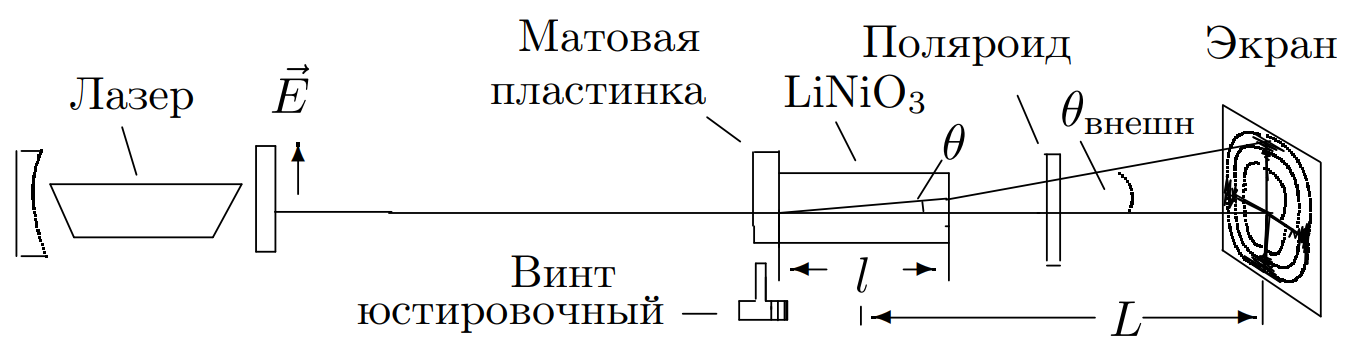
\includegraphics[width=\linewidth]{Pictures/Установка}
		\caption{Схема для наблюдения интерференционной картины}
	\end{figure}


	Разность фаз между обыкновенной и необыкновенной волнами, приобретаемая при прохождении через кристалл длиной $l$, равна
	\begin{equation*}
		\Delta \varphi = \frac{2\pi}{\lambda} l (n_1 - n_2).
	\end{equation*}


	Для обыкновенного луча $n_1 = n_o$. Считая, что $n_e$ и $n_o$ отличаются незначительно, для малых углов $(\sin\theta \approx \theta, \cos\theta \approx 1 - \theta^2/2)$ получаем $n_2$ = $n_o - (n_o - n_e)\theta^2$. Таким образом,
	\begin{equation*}
		\delta = \frac{2\pi}{\lambda}l(n_o - n_e)\theta^2.
	\end{equation*}


	Если $L$ -- расстояние от центра кристалла до экрана, то, учитывая закон преломления (закон Снеллиуса) на границе кристалла, при малых углах $\theta_{\text{внешн}} = n_o \theta$ (рис. 1) получаем выражение для радиуса кольца:
	\begin{equation*}
		r_m^2 = \frac{\lambda}{l}\frac{(n_o L)^2}{(n_o - n_e)}m.
	\end{equation*}


	При перпендикулярных ориентациях лазера и анализатора имеем:
	\begin{equation*}
		I_{\text{вых}} = I_0\sin^2\left(\frac{\pi}{2}\frac{U}{U_{\lambda / 2}}\right), 
	\end{equation*}
	где $U_{\lambda / 2} = \frac{\lambda}{4A} \frac{d}{l}$ -- полуволновое напряжение.

	При параллельных:
	\begin{equation*}
		I_{\text{вых}} = I_0\cos^2\left(\frac{\pi}{2}\frac{U}{U_{\lambda / 2}}\right).
	\end{equation*}

	\newpage

	\section*{Экспериментальная установка}
	\begin{figure}[h!]
		\centering
		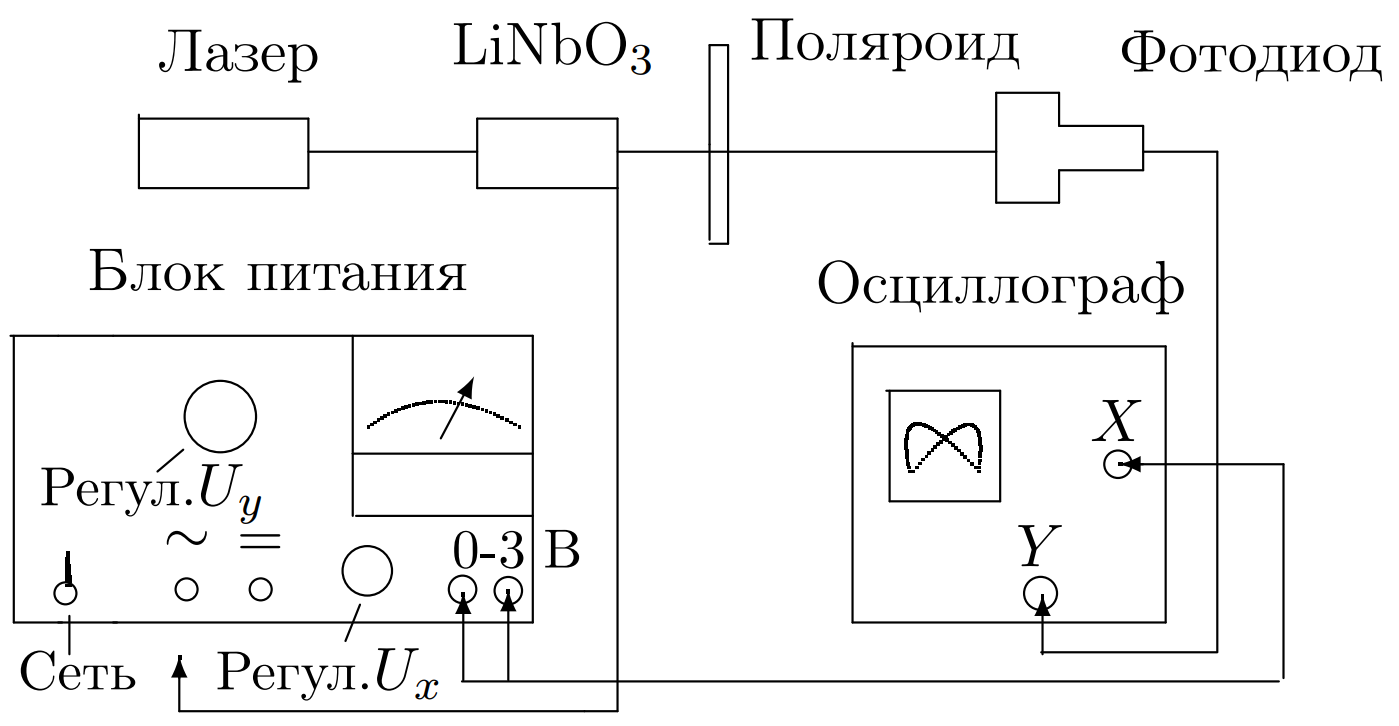
\includegraphics[width=\linewidth]{Pictures/Осциллограф}
		\caption{Схема для изучения двойного лучепреломления в электрическом поле}
	\end{figure}

	Оптическая часть установки представлена на рис. 1. Свет от гелий-неонового лазера, поляризованный в вертикальной плоскости, проходя сквозь матовую пластинку, рассеивается и падает на двоякопреломляющий кристалл под различными углами. Кристалл ниобата лития с размерами 3 $\times$ 3 $\times$ 26 мм вырезан вдоль оптической оси $Z$. На экране, расположенном за скрещенным поляроидом, видна интерференционная картина. Для $\lambda$ = 0,63 мкм (длина волны гелий-неонового лазера) в ниобате лития $n_o$ = 2,29.
	
	Убрав рассеивающую пластинку и подавая на кристалл постоянное напряжение, можно величиной напряжения влиять на поляризацию луча, вышедшего из кристалла.
	Заменив экран фотодиодом (рис. 2) и подав на кристалл переменное напряжение, можно исследовать поляризацию луча с помощью осциллографа.
	
	\newpage
	
	\section*{Ход работы}
	
	\begin{center}
		\textbf{I. Юстировка системы}
	\end{center}
	
	\begin{enumerate}
		\item Соберем оптическую схему согласно рис. 1. Включим лазер и установим анализатор так, чтобы лазерное излучение через него не проходило. 
		
		Чтобы убедиться, что лазерный луч поляризован вертикально, определим разрешённое направление анализатора: посмотрим сквозь поляроид на дневной свет от окна, отражённый от светлой поверхности; вращая поляроид, найдем минимум освещённости и заметим отсчёт угла на лимбе. Вблизи угла Брюстера в отражённом свете преобладает компонента светового вектора, параллельная плоскости стола («правило иголки»), следовательно, минимум отражённого света соответствует вертикальному разрешённому направлению поляроида.
		
		
		\item Поставим кристалл и установим перед ним вплотную к кювете матовую пластинку. Расстояние от кристалла до экрана определяет размер интерференционной картины и её контрастность. В нашем случае $L = 65$ см.
		
		\item Получим на экране интерференционную картину. Отклоняя кристалл с помощью юстировочного винта (рис. 1) и поворачивая рейтер с кюветой вокруг вертикальной оси, добьемся совмещения центра коноскопической картины с положением луча на экране в отсутствие матовой пластинки.
	
		Повернем анализатор на $90\degree$ и убедимся, что коноскопическая картина изменилась на негативную. Вернем анализатор в прежнее положение.

		\begin{center}
			\textbf{II. Измерения и обработка результатов}
		\end{center}
	
		\item Измерим радиусы тёмных колец $r(m)$ и расстояние $L$ от середины кристалла до экрана: $\boxed{L = (65,0 \pm 0,1) \text{ см}}$
		
		Результаты заносим в таблицу 1:
		\begin{table}[h!]
			\centering
			\begin{tabular}{|c|c|c|c|c|c|c|}
				\hline
				$m$        & 1   & 2   & 3   & 4   & 5   & 6   \\ \hline
				$r(m)$, см & 1,2 & 2,8 & 3,7 & 4,3 & 4,8 & 5,1 \\ \hline
			\end{tabular}
			\caption{Зависимость $r(m)$}
		\end{table}		
	
		
		\newpage
		Построим график $r^2 = f(m)$.
		
		\begin{figure}
			\centering
			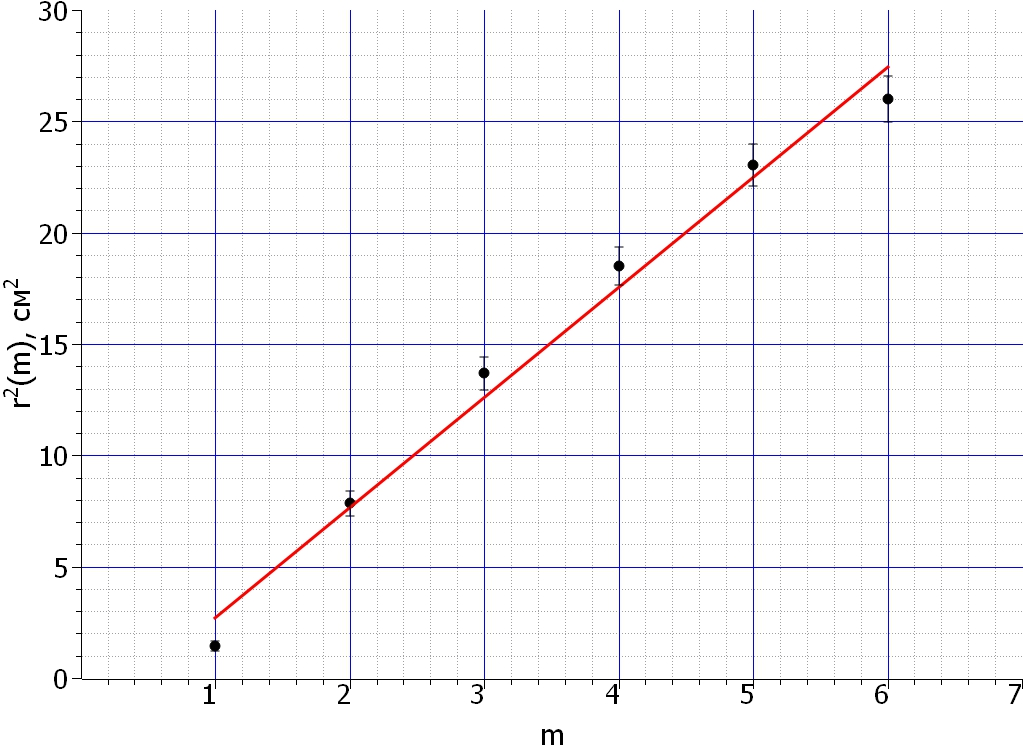
\includegraphics[width=0.8\linewidth]{Pictures/r2(m)}
			\caption{Зависимость $r(m)$}
		\end{figure}
	
	
		По углу наклона прямой определим двулучепреломление $(n_o - n_e)$ ниобата лития.
		
		Из графика получаем коэффициент наклона $\boxed{k = (5,2 \pm 0,3) \text{ см}^2}$
		
		Тогда:
		\begin{equation*}
			n_o - n_e = \frac{\lambda}{l}\frac{(n_o L)^2}{k},
		\end{equation*}
		где $l = 0,026$ м -- длина кристалла, а остальное нам дано.
		
		
		Получаем $\boxed{n_o - n_e = (1,03 \pm 0,07)}$. 
		
		Табличное значение $\thicksim 0,9$, что очень близко к нашему опыту.
		
		
		\item Подключим разъём блока питания на постоянное напряжение $(=)$, установим регулятор напряжения на минимальное напряжение и включим блок питания в сеть. С увеличением напряжения на кристалле яркость пятна на экране увеличивается и достигает максимума при $U = U_{\lambda / 2}$. При $U = 2U_{\lambda / 2} = U_\lambda$ яркость снова будет минимальной и т. д.
		Измерим $U_{\lambda / 2}$ и $U_\lambda$ для перпендикулярных и параллельных направлениях поляризатора и анализатора.
		
		\circled{$\perp$} $\hspace*{20mm} \boxed{U_{\lambda / 2} = (585 \pm 15) \text{ В}} \hspace*{30mm}  \boxed{U_{\lambda} = (1170 \pm 15) \text{ В}}$
		
		\circled{$\parallel$} $\hspace*{20mm} \boxed{U_{\lambda / 2} = (585 \pm 15) \text{ В}} \hspace*{30mm}  \boxed{U_{\lambda} = (1140 \pm 15) \text{ В}}$
		
		
		\item Подадим на кристалл так называемое четвертьволновое напряжение $U_{\lambda / 4} = \frac{1}{2} U_{\lambda / 2} = 293$ В. Поляризация на выходе кристалла должна быть круговой. Убедимся в этом, вращая анализатор и наблюдая за яркостью пятна на экране. Она не изменяется, поэтому и заключаем, что поляризация круговая.
		
		\item Установим вместо экрана фотодиод (рис. 2) и подключим его к $Y$-входу осциллографа. Убрав напряжение до нуля, переключим разъём с постоянного $(=)$ на переменное напряжение $(\sim)$. С трёхвольтового выхода блока питания подадим сигнал на вход $X$ осциллографа. Отклонение луча осциллографа по оси $X$, таким образом, будет пропорционально напряжению $U$ на кристалле, а по оси $Y$ -- интенсивности прошедшего через анализатор сигнала $I_{\text{вых}}$.
		
		
		\item Постепенно повышая напряжение на кристалле, наблюдаем на экране осциллографа фигуры Лиссажу, соответствующие зависимости $I_{\text{вых}}(U)$ для скрещенных поляризаций лазера и анализатора.
		
		Определим по фигурам Лиссажу полуволновое напряжение $U_{\lambda / 2}$ как $\Delta U$, соответствующее переходу от максимума к минимуму сигнала на осциллограмме: $\boxed{U_{\lambda / 2} = 600 \text{ В} }$
		
		\item Зарисуем фигуры Лиссажу для напряжений $U_{\lambda / 2}, U_\lambda, U_{3\lambda / 2}$ при скрещенных поляризациях лазера и анализатора.

		\begin{figure}[h!]
			\begin{minipage}[h]{0.3\linewidth}
				\center{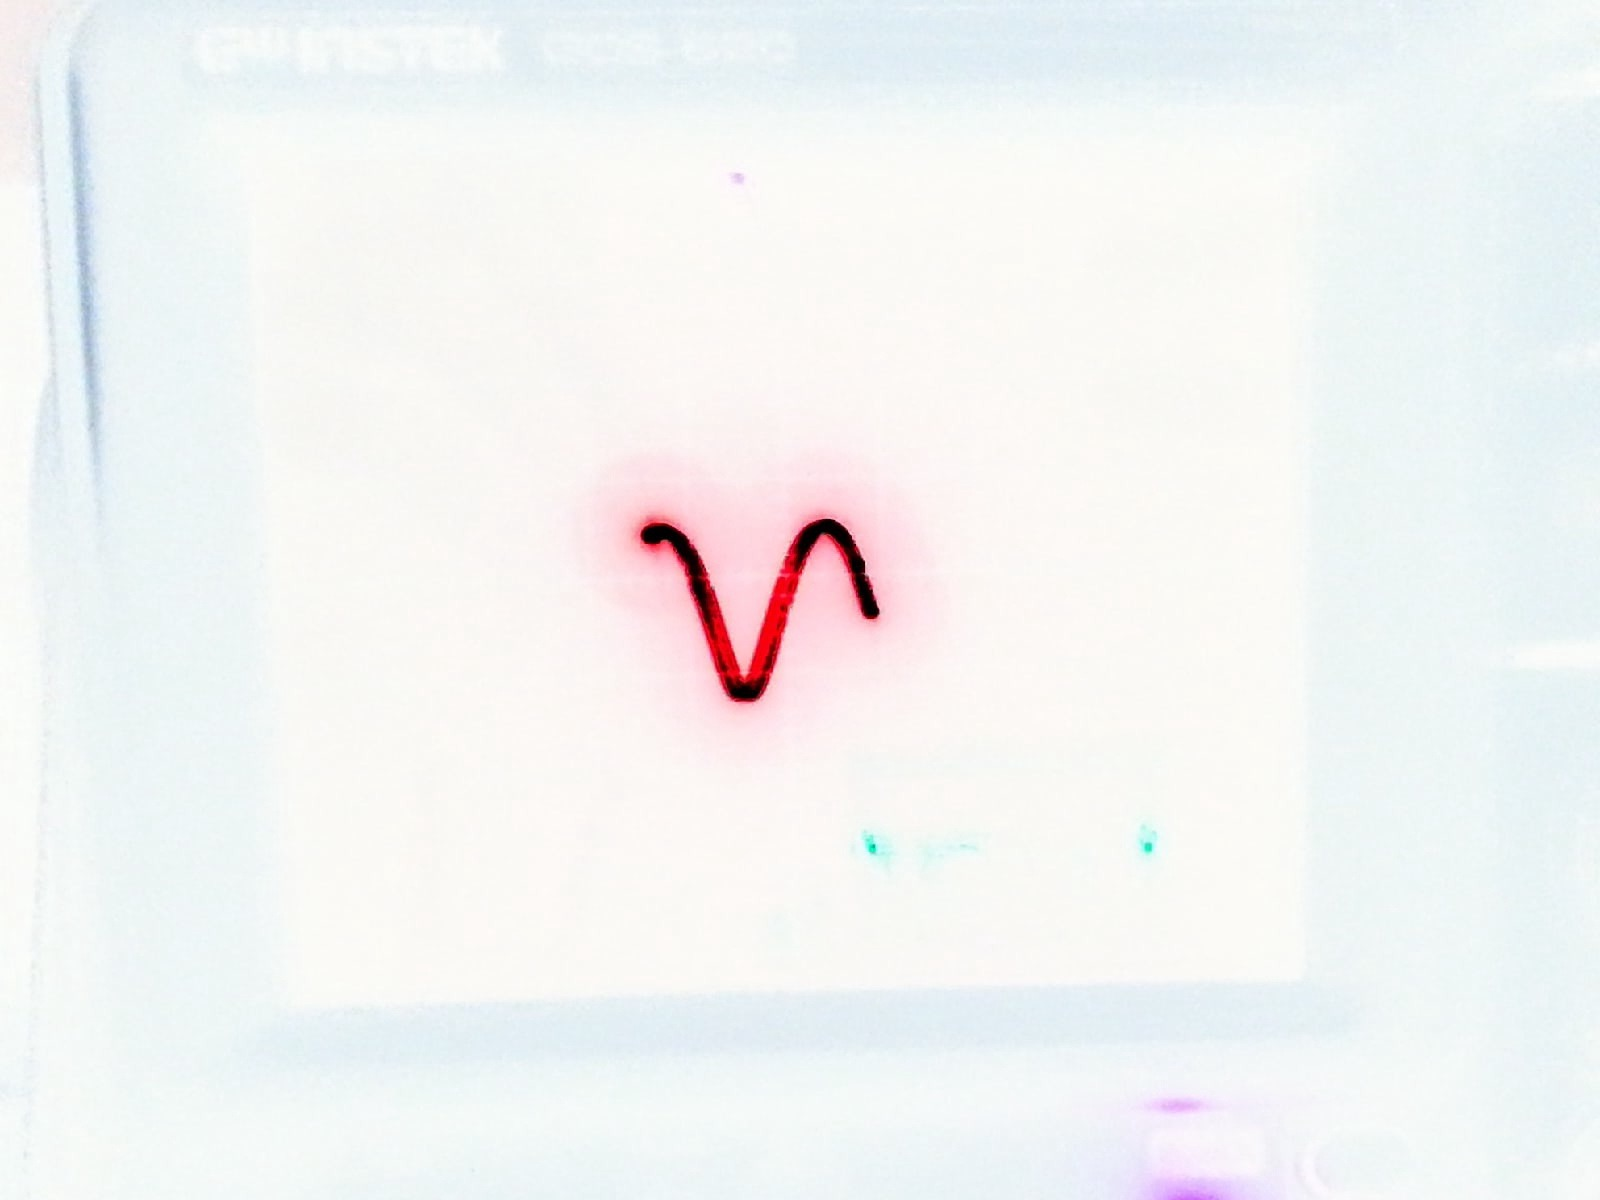
\includegraphics[width=\linewidth]{Pictures/Half} а)}
			\end{minipage}
			\hfill
			\begin{minipage}[h]{0.3\linewidth}
				\center{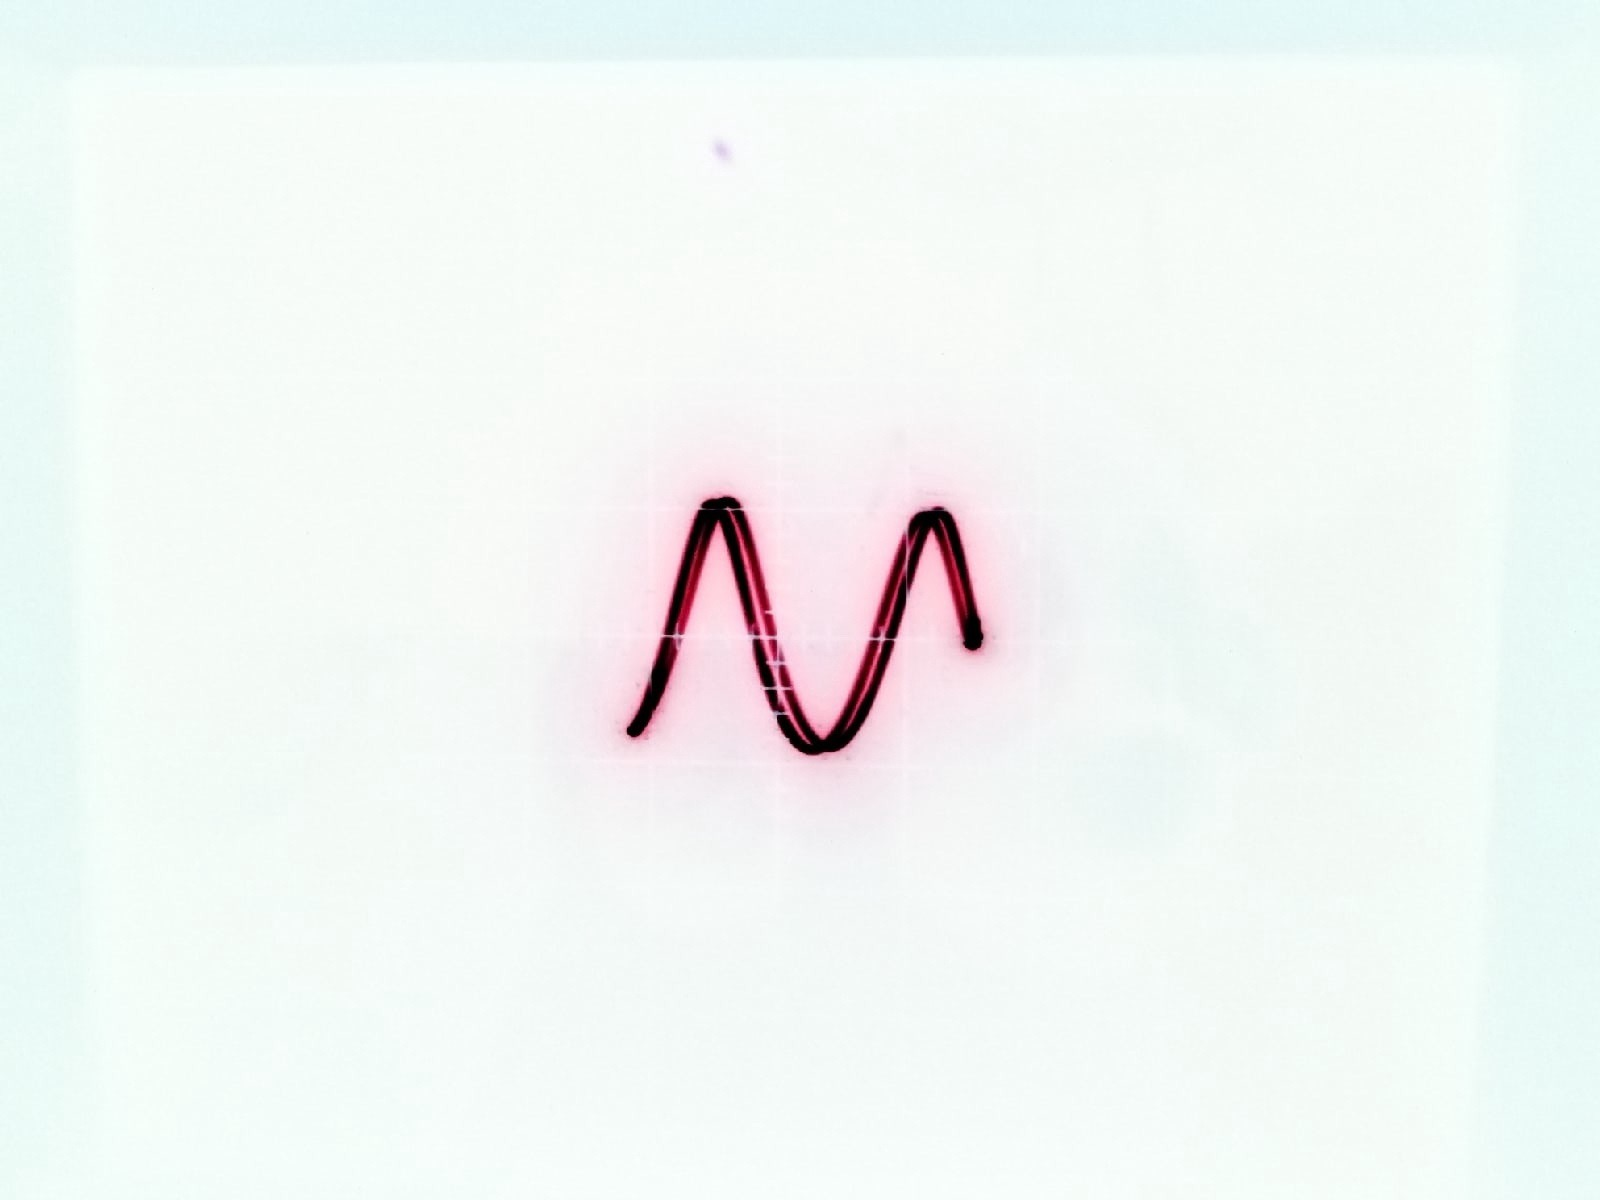
\includegraphics[width=\linewidth]{Pictures/Whole} б)}
			\end{minipage}
			\hfill
			\begin{minipage}[h]{0.3\linewidth}
				\center{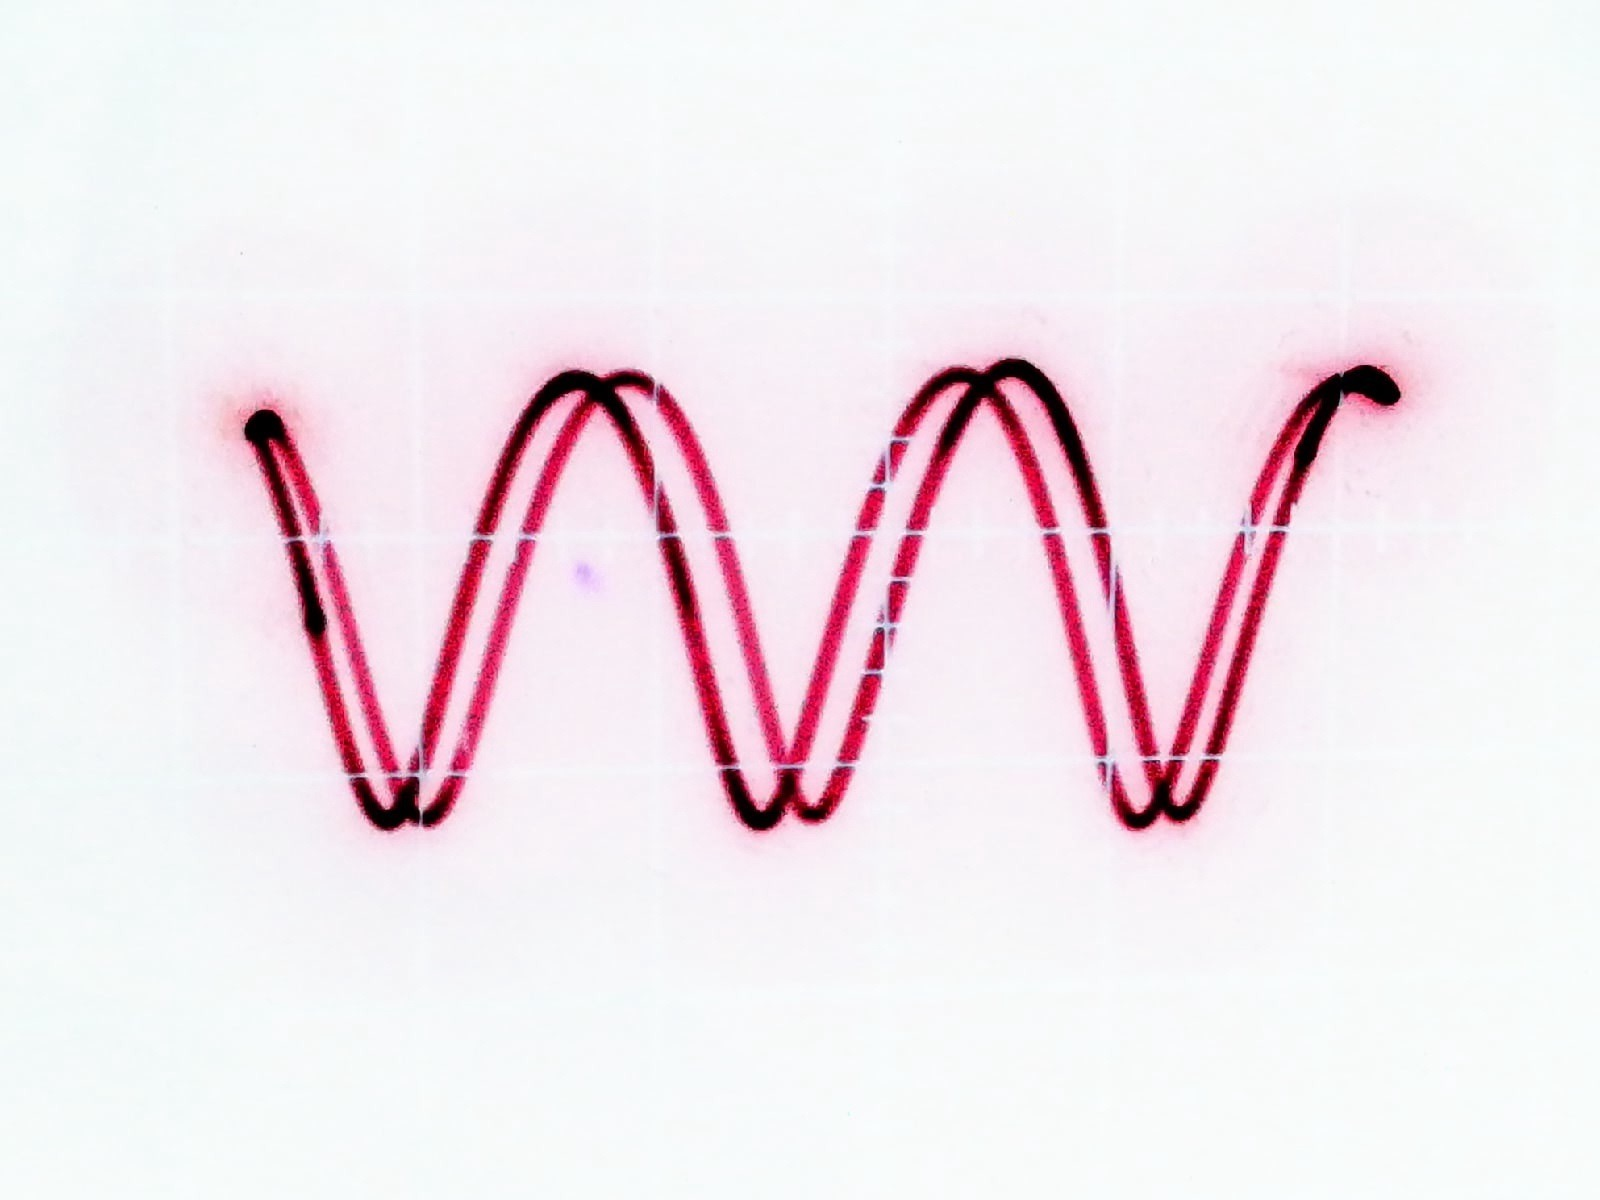
\includegraphics[width=\linewidth]{Pictures/ThreeHalves} в)}
			\end{minipage}
		\caption{Фигуры Лиссажу при напряжениях: а) $U_{\lambda / 2}$; б) $U_\lambda$; в) $U_{3\lambda / 2}$}
		\end{figure}
	\end{enumerate}

	\newpage
	\section*{Вывод}
	В работе была исследована интерференция рассеянного света, прошедшего кристалл. Было определено двойное лучепреломление для кристалла LiNbO$_3$: $n_o - n_e = (1,03 \pm 0,07)$, что согласуется с табличным значением в 0,9. Также мы пронаблюдали эффект Поккельса и нашли полуволновое напряжение кристалла: $U_{\lambda / 2} = (590 \pm 22)$ В. Присутствуют ошибки порядка $\thicksim 7\%$, что достаточно хорошо. Эти ошибки связаны с несовершенством техники измерений в работе.

\end{document}